% Created 2016-01-14 Thu 00:14
\documentclass[11pt]{article}
\usepackage[utf8]{inputenc}
\usepackage[T1]{fontenc}
\usepackage{fixltx2e}
\usepackage{graphicx}
\usepackage{longtable}
\usepackage{float}
\usepackage{wrapfig}
\usepackage{rotating}
\usepackage[normalem]{ulem}
\usepackage{amsmath}
\usepackage{textcomp}
\usepackage{marvosym}
\usepackage{wasysym}
\usepackage{amssymb}
\usepackage{hyperref}
\tolerance=1000
\usepackage[utf8]{inputenc}
\usepackage{commath}
\usepackage{pgf}
\usepackage{tikz}
\usetikzlibrary{shapes,backgrounds}
\usepackage{marginnote}
\usepackage{listings}
\usepackage{enumerate}
\usepackage{algpseudocode}
\usepackage{algorithm}
\usepackage{mathtools}
\usetikzlibrary{arrows,automata}
\setlength{\parskip}{16pt plus 2pt minus 2pt}
\renewcommand{\arraystretch}{1.6}
\DeclareMathOperator{\Neg}{Neg}
\author{Oleg Sivokon}
\date{\textit{<2016-01-01 Fri>}}
\title{Assignment 15, Authomata Theory}
\hypersetup{
  pdfkeywords={Automata Theory, Formal Languages, Assignment},
  pdfsubject={Fifth assignment in the course 20440 Automata and Formal Languages},
  pdfcreator={Emacs 24.5.1 (Org mode 8.2.10)}}
\begin{document}

\maketitle
\tableofcontents


\definecolor{codebg}{rgb}{0.96,0.99,0.8}
\definecolor{codestr}{rgb}{0.46,0.09,0.2}
\lstset{%
  backgroundcolor=\color{codebg},
  basicstyle=\ttfamily\scriptsize,
  breakatwhitespace=false,
  breaklines=false,
  captionpos=b,
  framexleftmargin=10pt,
  xleftmargin=10pt,
  framerule=0pt,
  frame=tb,
  keepspaces=true,
  keywordstyle=\color{blue},
  showspaces=false,
  showstringspaces=false,
  showtabs=false,
  stringstyle=\color{codestr},
  tabsize=2
}
\lstnewenvironment{maxima}{%
  \lstset{%
    backgroundcolor=\color{codebg},
    escapeinside={(*@}{@*)},
    aboveskip=20pt,
    captionpos=b,
    label=,
    caption=,
    showstringspaces=false,
    frame=single,
    framerule=0pt,
    basicstyle=\ttfamily\scriptsize,
    columns=fixed}}{}
}
\makeatletter
\newcommand{\verbatimfont}[1]{\renewcommand{\verbatim@font}{\ttfamily#1}}
\makeatother
\verbatimfont{\small}%
\clearpage

\section{Problems}
\label{sec-1}

\subsection{Problem 1}
\label{sec-1-1}
Given context-free grammar $V = \{S,M,N,W,X,Y,Z\}$ s.t. $T=\{1,0\}$

\begin{align*}
  &S \to M \;|\; XN \;|\; W \;|\; 0N \;|\; 1Z1 \\
  &M \to 0M0 \;|\; N \\
  &N \to N0 \;|\; 0 \\
  &W \to 0W \;|\; 00W0 \\
  &X \to 0X1 \;|\; 0 \;|\; 0Y0 \\
  &Z \to W \;.
\end{align*}


\begin{enumerate}
\item Is $V$ ambiguous?
\item Give a normalized grammar equivalent to $V$.
\end{enumerate}

\subsubsection{Answer 2}
\label{sec-1-1-1}
It is easier to normalize the grammar first and then to look for ambiguities,
thus the answers are in reverse order.
\begin{enumerate}
\item Any derivation containing $W$ cannot terminate, and so does $Z$.
\item Further, we can eliminate the rule $M \to N$.
\item $Y$ has no derivation rules, thus we can also remove it.
\end{enumerate}

Thus obtaining:
\begin{align*}
  &S \to M \;|\; XM \;|\; 0M \\
  &M \to 0M0 \;|\; 0 \;|\; 0M \\
  &X \to 0X1 \;|\; 0 \;.
\end{align*}

\begin{enumerate}
\item It is easy to see that $M$ derives number of zeros greater than one,
thus $M \to 0M0$ is redundant.  Subsequently, $S \to 0M$ is already
covered by $S \to M$.
\end{enumerate}


What remains is:
\begin{align*}
  &S \to M \;|\; XM \\
  &M \to 0 \;|\; 0M \\
  &X \to 0 \;|\; 0X1 \;.
\end{align*}

\subsubsection{Answer 1}
\label{sec-1-1-2}
Now it is easy to see that the string 00 can be derived in two different
ways:

\begin{itemize}
\item $S \to M$, $M \to 0M$, $M \to 0$.
\item $S \to XM$, $X \to 0$, $M \to 0$.
\end{itemize}

Hence $V$ is ambiguous.
\subsection{Problem 2}
\label{sec-1-2}
Given context-free grammar $V = \{S,M,N,W,X,Y,Z\}$ s.t. $T=\{1,0\}$

\begin{align*}
  &S \to 0W11 \;|\; 0X1 \;|\; 0Y \\
  &W \to S \;|\; Z \\
  &X \to S \;|\; W \\
  &Y \to 1 \\
  &Z \to X \;.
\end{align*}


\begin{enumerate}
\item Bring $V$ to Chomsky's normal form.
\item What is the language of $V$?
\end{enumerate}

\subsubsection{Answer 3}
\label{sec-1-2-1}
\begin{enumerate}
\item We can easily eliminate $Y$ variable, thus removing $Y \to 1$ rule,
and adding $S \to 01$ rule.
\item We can eliminate $Z$ variable by removing $Z \to X$ and $W \to Z$ rules
and adding $W \to X$ rule.
\item We can eliminate $X$ variable by removing $X \to S \;|\; W$ and $S \to
       0X1$ rules, and adding: $S \to 0S1$ rule.
\item Finally, we can eliminate $W$ variable by removing $W \to S$ and $S \to
       0W11$ rules and adding $S \to 0S11$ rule.
\end{enumerate}


The resulting grammar will be:

\begin{align*}
  &S \to 0S11 \;|\; 0S1 \;|\; 01 \;.
\end{align*}


Since this is still not CNF, I introduce an extra variable: $X$ and
derivation rules $X \to 0$, $Y \to 1 \;|\; 11$ and $Z \to SY$ thus
obtaining:

\begin{align*}
  &S \to XZ \;|\; 01 \\
  &X \to 0 \\
  &Y \to 1 \;|\; 11 \\
  &Z \to SY \;.
\end{align*}


Which is in CNF.

\subsubsection{Answer 4}
\label{sec-1-2-2}
Using the results from the previous answer it is easy to see that
the language $L(V)=\{0^n1^k \;|\; n \leq k \land n,k > 0\}$.

\subsection{Problem 3}
\label{sec-1-3}
Build a PDA accepting the language $L$ by emptying the stack.

\begin{align*}
  L = \{ a^{i_1}b^{j_1}a^{i_2}b^{j_2}\dots a^{i_m}b^{j_m}
       &\;|\; m \geq 1 \\
       &\;|\; \forall k: i_k \geq j_k \geq 1 \\
       &\;|\; \exists k: i_k > j_k \}
\end{align*}

\subsubsection{Answer 5}
\label{sec-1-3-1}
First, I'll write the grammar for $L$ (because it's easier to do):

\begin{align*}
  &S \to aSb \;|\; K \;|\; SS \\
  &K \to aKb \;|\; aaKb \\
  &X \to aXb \;|\; aaXb \;|\; \epsilon \;.
\end{align*}

\begin{enumerate}
\item $X$ generates strings of the form $\{ a^nb^m \;|\; n \geq m \}$.
\item Similarly, $K$ generates strings of the form $\{ a^nb^m \;|\; n > m \}$.
\item The derivatin of $S$ can only terminate when it eventually derives either
$K$.  It can repeat as many times as needed to accept the entire string.
Where the repeated element is, again, of the form of either $\{ a^nb^m
        \;|\; n \geq m \}$, or  $\{ a^nb^m \;|\; n > m \}$.
\end{enumerate}

Thus, at least informally, we are convinced the grammar generates $L$.

Now, the automaton:

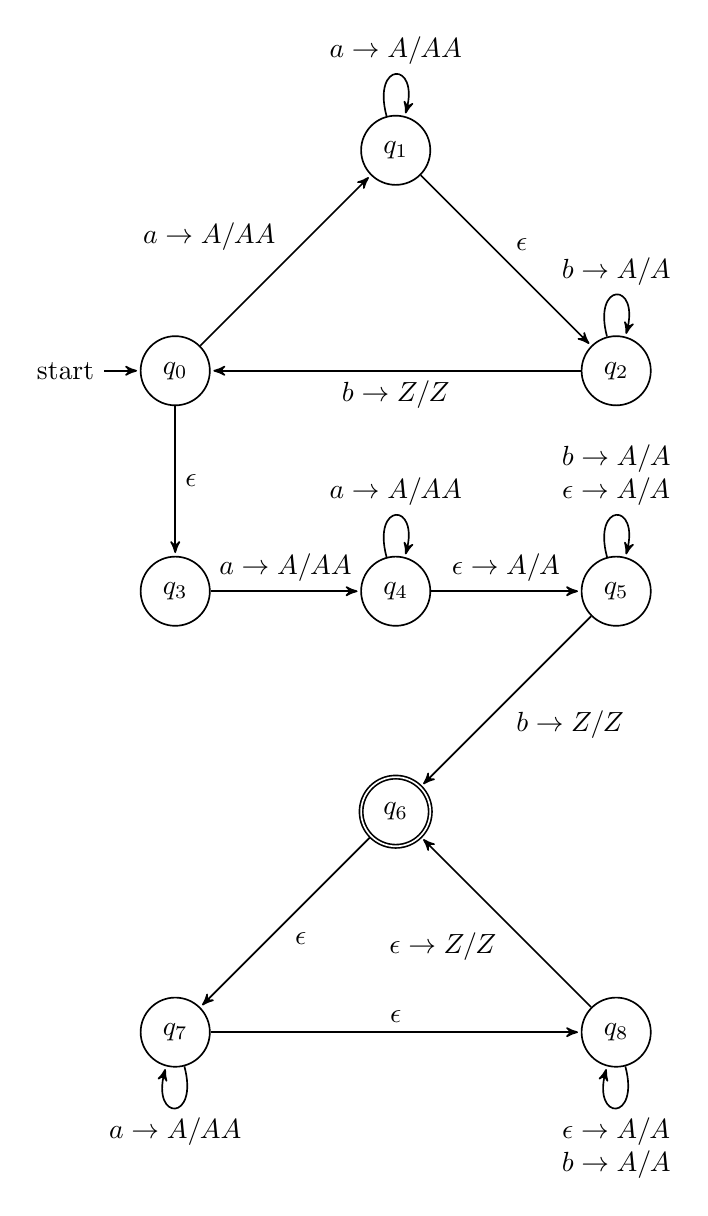
\begin{tikzpicture}[->,>=stealth',shorten >=1pt,auto,node distance=2.8cm,
                    semithick]

  \node[initial,state]   (A)              {$q_0$};
  \node[state]           (B) [right of=A, above of=A] {$q_1$};
  \node[state]           (C) [right of=B, below of=B] {$q_2$};
  \node[state]           (D) [below of=A] {$q_3$};
  \node[state]           (E) [right of=D] {$q_4$};
  \node[state]           (F) [right of=E] {$q_5$};
  \node[accepting,state] (G) [below of=E] {$q_6$};
  \node[state]           (H) [left of=G, below of=G] {$q_7$};
  \node[state]           (J) [right of=G, below of=G] {$q_8$};

  \path (A) edge              node {$a \to A/AA$} (B)
            edge              node {$\epsilon$} (D)
        (B) edge [loop above] node {$a \to A/AA$} (B)
            edge              node {$\epsilon$} (C)
        (C) edge [loop above] node {$b \to A/A$} (C)
            edge              node {$b \to Z/Z$} (A)
        (D) edge              node {$a \to A/AA$} (E)
        (E) edge [loop above] node {$a \to A/AA$} (E)
            edge              node {$\epsilon \to A/A$} (F)
        (F) edge [loop above, align=center] node {$b \to A/A$ \\ $\epsilon \to A/A$} (F)
            edge              node {$b \to Z/Z$} (G)
        (G) edge              node {$\epsilon$} (H)
        (H) edge [loop below] node {$a \to A/AA$} (G)
            edge              node {$\epsilon$} (J)
        (J) edge [loop below, align=center] node {$\epsilon \to A/A$ \\ $b \to A/A$} (J)
            edge              node {$\epsilon \to Z/Z$} (G);
\end{tikzpicture}

The idea behind this diagram is as follows:
\begin{enumerate}
\item Loop as many times as needed (possibly zero) over strings $a^nb^n$, where
$n \geq 1$.
\item Nondeterministically parse a string $a^nb^m$ where $n > m$.
\item Loop as many times as needed (possibly zero) over strings $a^nb^m$ where
$n \geq m$.
\item Before accepting state, keep discarding $A$ until none remain for as long as
you don't see an $a$.
\item Accept the string.
\end{enumerate}
% Emacs 24.5.1 (Org mode 8.2.10)
\end{document}
